\chapter{Kata Containers in telco environment}
\label{chapter:implementation}

\textcolor{red}{Come up with better chapter name}

Telco systems are a complex environment with multiple requirements for connectivity and performance. This chapter discusses the requirements of telco systems, implementation and possible limitations of Kata Containers in this environment. The performance and tests are described in Chapter \ref{chapter:evaluation}. The features discussed in this chapter are related to Kubernetes configurations.

\section{CPU}

Telecommunication applications are computing heavy, which require efficient usage of the resources. One of the requirements telco applications have for infrastructure is the support for core isolation. This feature allows to dedicate a single core to a process in order to minimize interruptions for the process. (Core isolation involves removes all user-space threads, unbound kernel threads, and blocks interruptions from the system \cite{CPUisolation}).

One option to dedicate a core for a process is defining a pod with a Quality of Service (QoS) class of Guaranteed and one CPU as resource \cite{QOSKubernetes}. This option allows the whole core to be dedicated for the container process. However, with Kata Containers the architecture includes a Kata-agent and a guest kernel for each pod as described in Figure \ref{fig:KataContainersComponents}. These resources need to be assigned to a second core, which can be a shared resource between other pods. The shared resources can also host general cluster components such as monitoring and DNS.



- Is core isolation possible?
	- Dedicated core to container
		- Improves the performance
	- Does agent or other process interrupt the core VM exits (or some other instruction)
	- Measuring
		- Implement busylooping app noticing time of execution
		- DPDK test apps

At what point the resources are allocated?

\section{Memory}

Telco systems rely on high-throughput and low-latency data sharing between containers and pods. Writing and reading a shared block of memory between containers offers the fastest way for shared information. In Kubernetes, containers can share IPC namespaces with the help of pod security policies \cite{PodSecurityPolicyKubernetes}. Configuration of these policies enable usage of HostIPC, which controls whether the pod containers can share host IPC namespace.

\textcolor{red}{How happened with Kata Containers?} \\
\textcolor{red}{Is it possible to share memory between pods inside a node? If not, is there a workaround} \\

Memory is managed in blocks known as pages. In most systems, the default page size is 4 kilobytes, thus 1 megabyte of memory equals to 256 pages. CPUs have built-in memory management unit managing a list of these pages in hardware. The management unit, Translation Lookaside Buffer (TLB), has a fixed number of pages it can store. Once the number of pages exceed the number of defined in TLB, the systems fails back to a slower, software-based address translation. This transition results in degraded performance. Since the number of pages stored in the TLB is fixed, the only way to increase a chance of TLB miss is to increase the page size with huge pages. \cite{HugePagesOpenShift}

\subsection{Huge pages}

Huge pages is a memory page with size larger than 4 kilobytes. In x86\_64 architectures the two common sizes are 2MB and 1GB. In order to use huge pages, the application must be developed to use the larger page sizes. The high performance telco applications also use huge pages, thus the support is crucial to maintain the performance.

Kubernetes supports the allocation and consumption of pre-allocated huge pages by applications in a pod \cite{HugePagesKubernetes}. Kata Containers also support using huge pages, however it needs to be specifically configured in a custom Kata Containers kernel. As Kata Containers architecture consumes more memory than a native design with runC, it is crucial that the pod is allocated enough resources to support huge pages.

\section{Storage}

High performance Kubernetes storage options are usually limited to storages which locate in nearby the computing unit. Thus, network storages or block storages hosted on commercial cloud, which rely on data transmission via network are not sufficient enough regarding performance. In telco systems, three types of storages are used for high-performance applications: emptyDir, hostPath, and local. EmptyDir is non-persistent volume, meaning it does not retain data stored if the attached pod is removed from a node. In contrast, hostPath and local storages are Persistent Volumes (PV), a Storage Class defined in Kubernetes. These storages are individual of restructing of the cluster architecture and thus are applicable for storing user related data or logs, whereas emptyDir is mainly used for session specific data or offloading memory temporarily.

\subsection{emptyDir}

An emptyDir volume is first created when a pod is assigned to a node, and exists as long as that Pod is running on that node. emptyDir volume is initially empty. All containers in the pod emptyDir is attached to can read and write the same files in the volume. Some use cases for emptyDir are scratch space during disk-based merge sort, checkpointing during a long computation in case of crashes, and holding files that a content-manager container fetches while a web server container serves the data. \cite{VolumesKubernetes}

EmptyDir volumes are stored on various medium that backs the such as disk or SSD. However, it supports also RAM-backed filesystem tmpfs, which offers very fast alternative to disk based volumes. However, tmpfs is cleared on node reboot and any data written on it counts against container's memory limit. \cite{VolumesKubernetes}

\subsection{Persistent Volume}

Persistent Volume is a piece of storage in the cluster has been provisioned dynamically or by an administrator. PVs are volume plugins having a lifecycle independent of any individual Pod using the PV. Kubernetes supports multiple types of persistent storage resources, such as Network Filesystem (NFS), SCSI over IP (iSCSI), local storage devices, or AWS Elastic Block Store \cite{AmazonEBS}. \cite{PV}

PV volumes can be mounted to nodes in Kubernetes with three different access modes: ReadWriteOnce, ReadOnlyMany, and ReadWriteMany. ReadWriteOnce allows only one node for read and write operations. ReadOnlyMany is read-only mode allowing multiple nodes for simultaneous access. In contrast, ReadWriteMany allow multiple nodes for simultaneous read and write operations. PVs have different support for read and write options. In this Thesis, we will focus on two PV options, which are hostPath and local. \cite{PV} 

\subsubsection{HostPath}

A hostPath volume mounts a file or directory from the host node's filesystem into the pod. Some use cases for hostPath include running a container that needs access to Docker internals or running cAdvisor in a container which requires an access to system directory. HostPath is only applicable inside a single node, however multiple pods can write simultaneously into the same file or directory.

\subsubsection{Local volume}

Local volume represents a mounted local storage device such as a disk, partition or directory \cite{VolumesKubernetes}. Local volumes can only be created statically, and dynamic provisioning is not supported. Compared to hostPath volumes, local volumes are used in a durable and portable manner without manually scheduling pods to nodes. Local volumes are subject to the availability of the underlying node. Downtime of the node including storage disables all access to the storage reducing availability, as possibly causing potential data loss.

Local volume can be mounted to the node as a filesystem or raw block device. These raw block volumes are mounted into a pod without any filesystems on it. The filesystem layer introduces unneeded overhead, thus some specialized applications require direct access to a block device to maximize performance. A common case is databases, which prefer to organize their data directly on the underlying storage. Raw block devices are also commonly used by software which itself implements its storage service. \cite{RawBlockKubernetes}

%local with multiple access?
%Limitations? \\

\section{Network}

Kubernetes networking supports a feature for sharing process namespaces between containers in a pod. When process namespace sharing is enabled, processes in a container are visible to other containers in that pod. This feature is highly useful to configure cooperating containers, such as log handler sidecar container, or to troubleshoot container images that do not include debugging utilities like a shell. Process Namespace Sharing is enabled in the pod configuration in Kubernetes. This feature also enables to signal processes in other containers. For example, SIGHUP can be sent to nginx to restart the worker process. SYS\_PTRACE capability is required to enable signalling feature. \cite{ShareProcessNamespaceKubernetes}

In telco systems, shared network namespaces are used for interprocess communication through shared memory and unix sockets. This communication is vital for multiprocess applications, where each process handles a specific part of the business logic and need to communicate with each other. In telco environment, low-latency needs to be guaranteed, therefore the latency requirement is not satisfied using network based communication such as through IP. Kata Container supports process namespace sharing in the latest versions.

\subsection{Multus}

Telco networking requires connecting to multiple network simultaneously. By default, Kubernetes supports only a single network, apart from loopback, to be attached to a pod. In order extend the network interface, Multus CNI has been adopted to the cluster stack.

Multus CNI \cite{Multus} is a container network interface plugin for Kubernetes that enables attaching multiple network interfaces to pods. By default, in Kubernetes each pod has one network interface. With the help of Multus, pods can be multi-homed and attached with multiple interfaces. Figure \ref{fig:Multus} demonstrates a Multus enabled pod setup with two networks in Kubernetes. The pod includes three interfaces: net0, net1, and eth0. Network attachments net0 and net1 connect to outbound services by using CNI plugins such as vlan, vxlan, or ptp. eth0 interface connects to Kubernetes cluster network to connect with the server or services such as kubernetes-api-server or kubelet. Enabling Multus for Kata Containers environment is supported and requires no extra configuration apart from the Kubernetes configuration. In some environments Persistent Volume is required to enable Multus CNI \cite{MultusUbuntu}.

\begin{figure}[ht]
  \begin{center}
    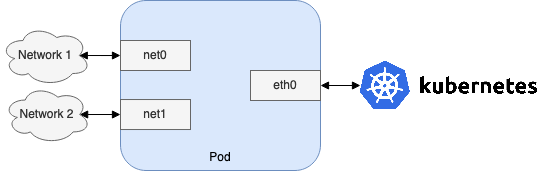
\includegraphics[width=13.5cm]{images/Multus.png}
    \caption{Multus enabled pod with two networks}
    \label{fig:Multus}
  \end{center}
\end{figure}

\subsection{SR-IOV}
\label{section:SR-IOV}

I/O throughput is critical to high performance telco systems. I/O intensive servers may waste CPU cycles, waiting for I/O data or spinning on idle cycles, which reduces system performance and increases latency. Single Root I/O Virtualization (SR-IOV) standard allows an I/O device, such as network interface controller (NIC), to be shared by multiple VMs. The SR-IOV technology is a hardware based virtualization solution that improves both performance and scalability. \cite{Dong2012}

Traditionally, when a guest accesses the I/O device, VMM needs to intervene in the data processing to share the physical device. The VMM intervention leads to additional I/O overhead for a guest OS. SR-IOV provides hardware enhancements for the Peripheral Component Interconnect Express (PCIe) device, which aims to remove major VMM intervention for performance data movement, such as the packet classification and address translation. An SR-IOV-capable device is able to create multiple light-weight instances of PCI function entities, known as Virtual Functions (VF). Each VF can be assigned to a VM for direct access, but still shares major device resources, achieving both resource sharing and high performance. \cite{Dong2012}

In Kubernetes, Kata Containers supports SR-IOV with a CNI plugin \cite{SR-IOVOpenShift}. Additionally, the Kata runtime detects virtual functions in container's network namespace to use SR-IOV for network based devices. In order to enable SR-IOV with Kata, a specific Docker plugin needs to be installed. The created network is based on a physical function device. \cite{SR-IOVKataContainers}

In order to setup host for SR-IOV, the system needs to support Intel Virtualization Technology for Directed I/O (VT-d) and the NIC device needs to support SR-IOV. Also, the host kernel must have Input-Output Memory Management Unit (IOMMU) and Virtual Function I/O (VFIO) support.

- SR-IOV \\
	- Multus needs to be accessible from Kata guest hosts \\
	
- If SR-IOV is accessible, the network performance remains the same
	- If not and using virtio, and hypervisor between nw performance might degrade
		- Measure throughput and latency between pods with iPerf (client - server)

\subsection{Hardware acceleration}

Hardware acceleration is the use of hardware specifically crafted to perform some functions more efficiently than software running on general-purpose CPUs. Hardware accelerated process can highly enhance the performance of cloud workloads by increasing throughput and decreasing latency and energy consumption. Hardware acceleration can be usage of GPUs for computing, SmartNIC \cite{SmartNICIntel}, or purpose built application-specific integrated circuit (ASIC) such as System on a Chip (SoC).

The main use of hardware acceleration for edge cloud environment is GPUs. Kata Containers supports passing certain GPUs from to host into the container using GPU passthrough as well as GPU mediated passthrough. GPU passthrough, such as Intel GVT-d, allows direct assignment of an entire GPU to a single user, passing the native driver capabilities through the hypervisor without any limitations. Mediated GPU passthrough, such as Intel GVT-g with multiple VMs to one physical GPU, is a full GPU virtualization solution with mediated pass-through.
A virtual GPU instance is maintained for each VM, with part of performance critical resources, directly assigned. The ability to run a native graphics driver inside a VM without hypervisor intervention in performance critical paths, achieves a good balance among performance, feature, and sharing capability. \cite{GPUKataContainers}
		
\section{Logging}

Kata Containers provides the workload with guest kernel, meanwhile the host uses dedicated kernel, which are not connected. One benefit of the architectural change in comparison to standard container workloads is the availability in case of kernel crashes. This availability is highly beneficial for logging purposes, as the crash of worker container does not wipe all logs at the same time.

\section{Limitations}